% !TEX root = ./document.tex

\documentclass{article}
\usepackage{mystyle}
\usepackage{myvars}


%-----------------------------

\begin{document}

	\maketitle
	\thispagestyle{firststyle}


%-----------------------------
%	ABSTRACT
%-----------------------------

	\begin{abstract}
		\noindent [TODO ]
	\end{abstract}

%-----------------------------
%	TEXT
%-----------------------------


	\section{Introduction}
	\label{sec:intro}

			\paragraph{}
			[TODO ]


	\section{Supervised Learning}
	\label{sec:supervised-learning}

		\paragraph{}
		[TODO ]

		\paragraph{Error Measures}
		\label{paragraph:error-measures}
		[TODO ]

		\begin{itemize}
			\item
				\textbf{Error Rate}:
				[TODO ]

			\item
				\textbf{Resubstitution error}:
				[TODO ]

			\item
				\textbf{Generalization Error}:
				[TODO ]

		\end{itemize}

		\paragraph{Experimental Strategies}
		\label{paragraph:experimental-strategies}
  	[TODO ]

		\begin{itemize}
			\item
				\textbf{Holdout}:
				[TODO ]

			\item
				\textbf{Repeated Holdout}:
				[TODO ]

			\item
				\textbf{Cross Validation}:
				[TODO ]

			\item
				\textbf{Repeated Cross Validation}:
				[TODO ]

		\end{itemize}

		\subsection{Decision Trees}
		\label{sec:decision-trees}

			\paragraph{}
			[TODO ]


			\subsubsection{Information Theory}
			\label{sec:information-theory}

				\paragraph{}
				[TODO ]

			\subsubsection{ID3}
			\label{sec:id3-tree}

				\paragraph{}
				[TODO ]

			\subsubsection{C4.5}
			\label{sec:c45-trees}

				\paragraph{}
				[TODO ]

		\subsection{Rule Based Systems}
		\label{sec:decision-trees}

			\paragraph{}
			[TODO ]

			\subsubsection{1R}
			\label{sec:1r-rule-based}

				\paragraph{}
				[TODO ]

			\subsubsection{PRISM}
			\label{sec:prism-rule-based}

				\paragraph{}
				[TODO ]

			\subsubsection{IREP}
			\label{sec:irep-rule-based}

				\paragraph{}
				[TODO ]

			\subsubsection{RIPPER}
			\label{sec:ripper-rule-based}

				\paragraph{}
				[TODO ]

			\subsubsection{PART}
			\label{sec:part-rule-based}

				\paragraph{}
				[TODO ]

		\subsection{Instance Based Learning}
		\label{sec:decision-trees}

			\paragraph{}
			[TODO ]

			\subsubsection{K - Nearest Neighbors}
			\label{sec:knn}

				\paragraph{}
				[TODO ]

			\subsubsection{IB3}
			\label{sec:ib3}

				\paragraph{}
				[TODO ]

		\subsection{Bayes Learning}
		\label{sec:decision-trees}

			\paragraph{}
			[TODO ]

			\subsubsection{Naive Bayes}
			\label{sec:naive-bayes}

				\paragraph{}
				[TODO ]

			\subsubsection{K2}
			\label{sec:k2-bayes}

				\paragraph{}
				[TODO ]

			\subsubsection{TAN}
			\label{sec:tan-bayes}

				\paragraph{}
				[TODO ]

		\subsection{Linear Classifiers}
		\label{sec:decision-trees}

			\paragraph{}
			[TODO ]

			\subsubsection{Linear Regression}
			\label{sec:linear-regression}

				\paragraph{}
				[TODO ]

			\subsubsection{Logistic Regression}
			\label{sec:logistic-regression}

				\paragraph{}
				[TODO ]

			\subsubsection{Support Vector Machines}
			\label{sec:svm}

				\paragraph{}
				[TODO ]


		\subsection{Neural Networks}
		\label{sec:neural-networks}

			\subsubsection{Perceptron model}

			\begin{figure}
				\centering
				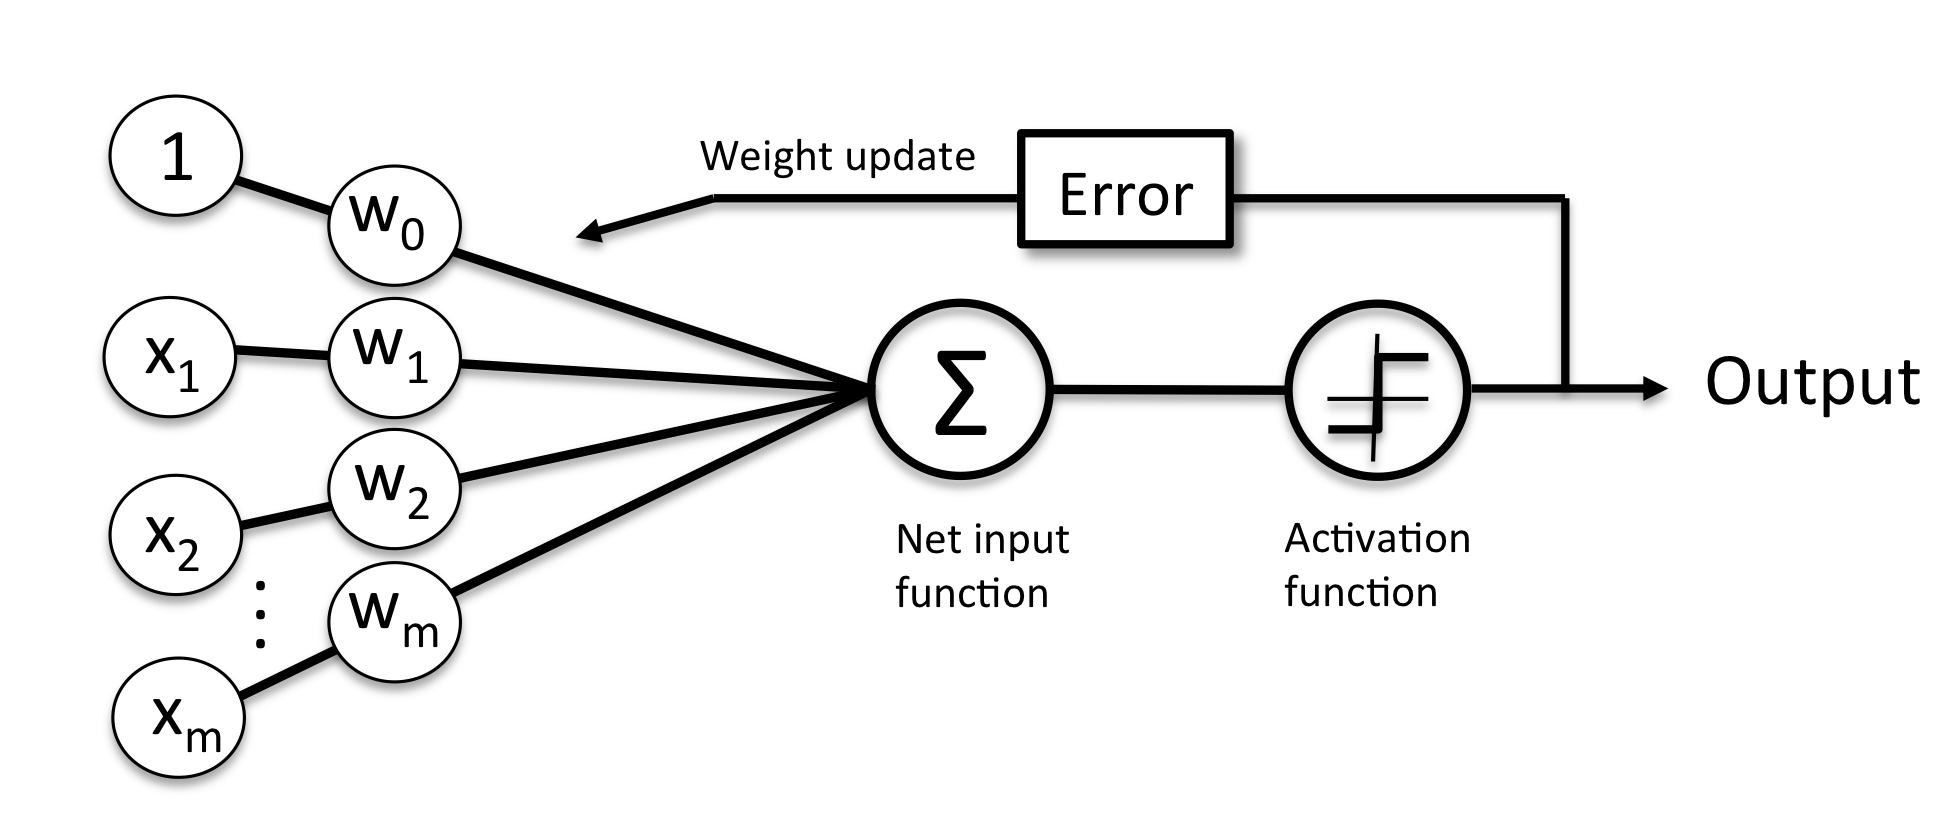
\includegraphics[width=.4\textwidth]{perceptron-concept}
				\caption{General concept of perceptron}
				\label{fig:perceptron-concept}
			\end{figure}

			\paragraph{Perceptron's structures}
			\begin{equation}
				w = \begin{bmatrix}
						w_1 \\
						\vdots \\
						w_m
					\end{bmatrix}, x =
					\begin{bmatrix}
						x_1 \\
						\vdots \\
						x_m
					\end{bmatrix}
			\end{equation}

			\paragraph{Ouput equation}
			\begin{equation}
				z = w_1 x_1 + \dots + w_m x_m = \boldsymbol{w^T x}
			\end{equation}


			\paragraph{Activation function}

			\begin{figure}
				\centering
				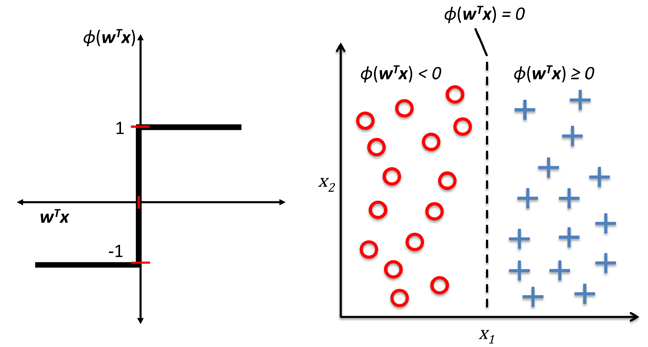
\includegraphics[width=.4\textwidth]{activation-function}
				\caption{Activation function}
				\label{fig:activation-function}
			\end{figure}

			\begin{equation}
				\phi(z) = \begin{cases}
					1 &\mbox{if } z \geq \theta \\
					-1 &\mbox{otherwise}
				\end{cases}
			\end{equation}

			\paragraph{Update of weight vector}

			\begin{align}
					w_j &:= w_j + \Delta w_j \\
					\Delta w_j &= \eta(y^{(i)} - \hat{y}^{(i)}) x^{(i)}_j
			\end{align}

			\subsubsection{Adaptive linear neurons (ADALINE)}

			\begin{figure}
				\centering
				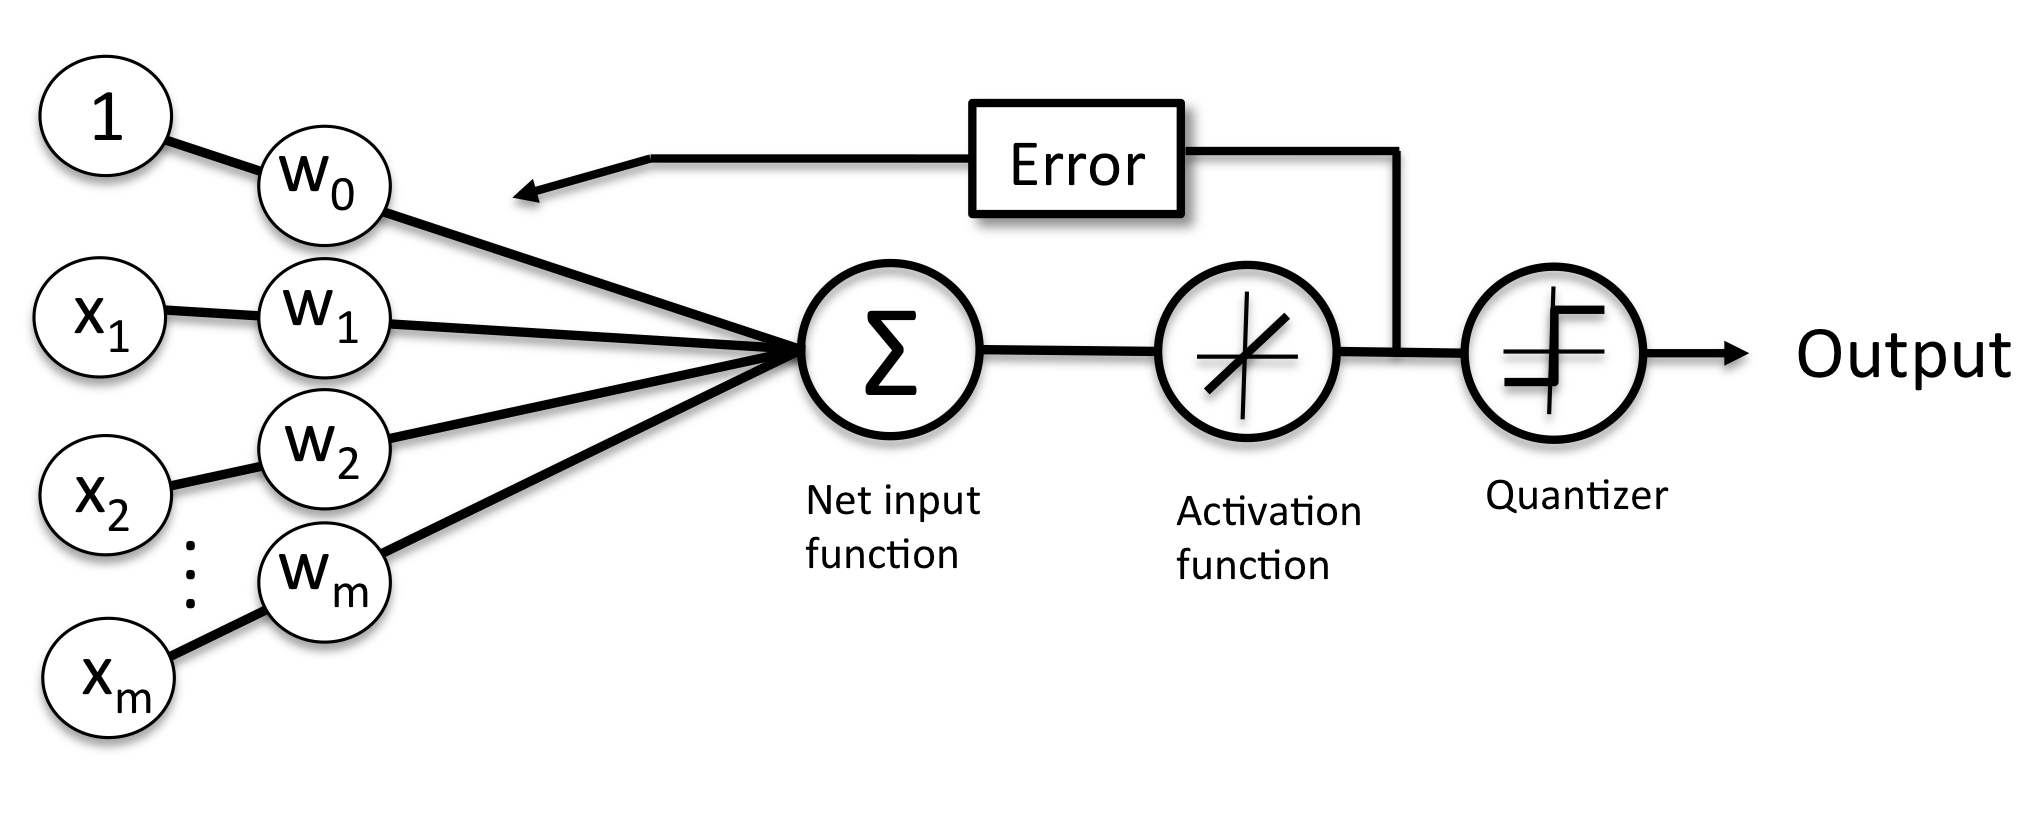
\includegraphics[width=.4\textwidth]{adaline-concept}
				\caption{General concept of adaline perceptron}
				\label{fig:adaline-concept}
			\end{figure}

			\paragraph{Cost function}

			\begin{figure}
				\centering
				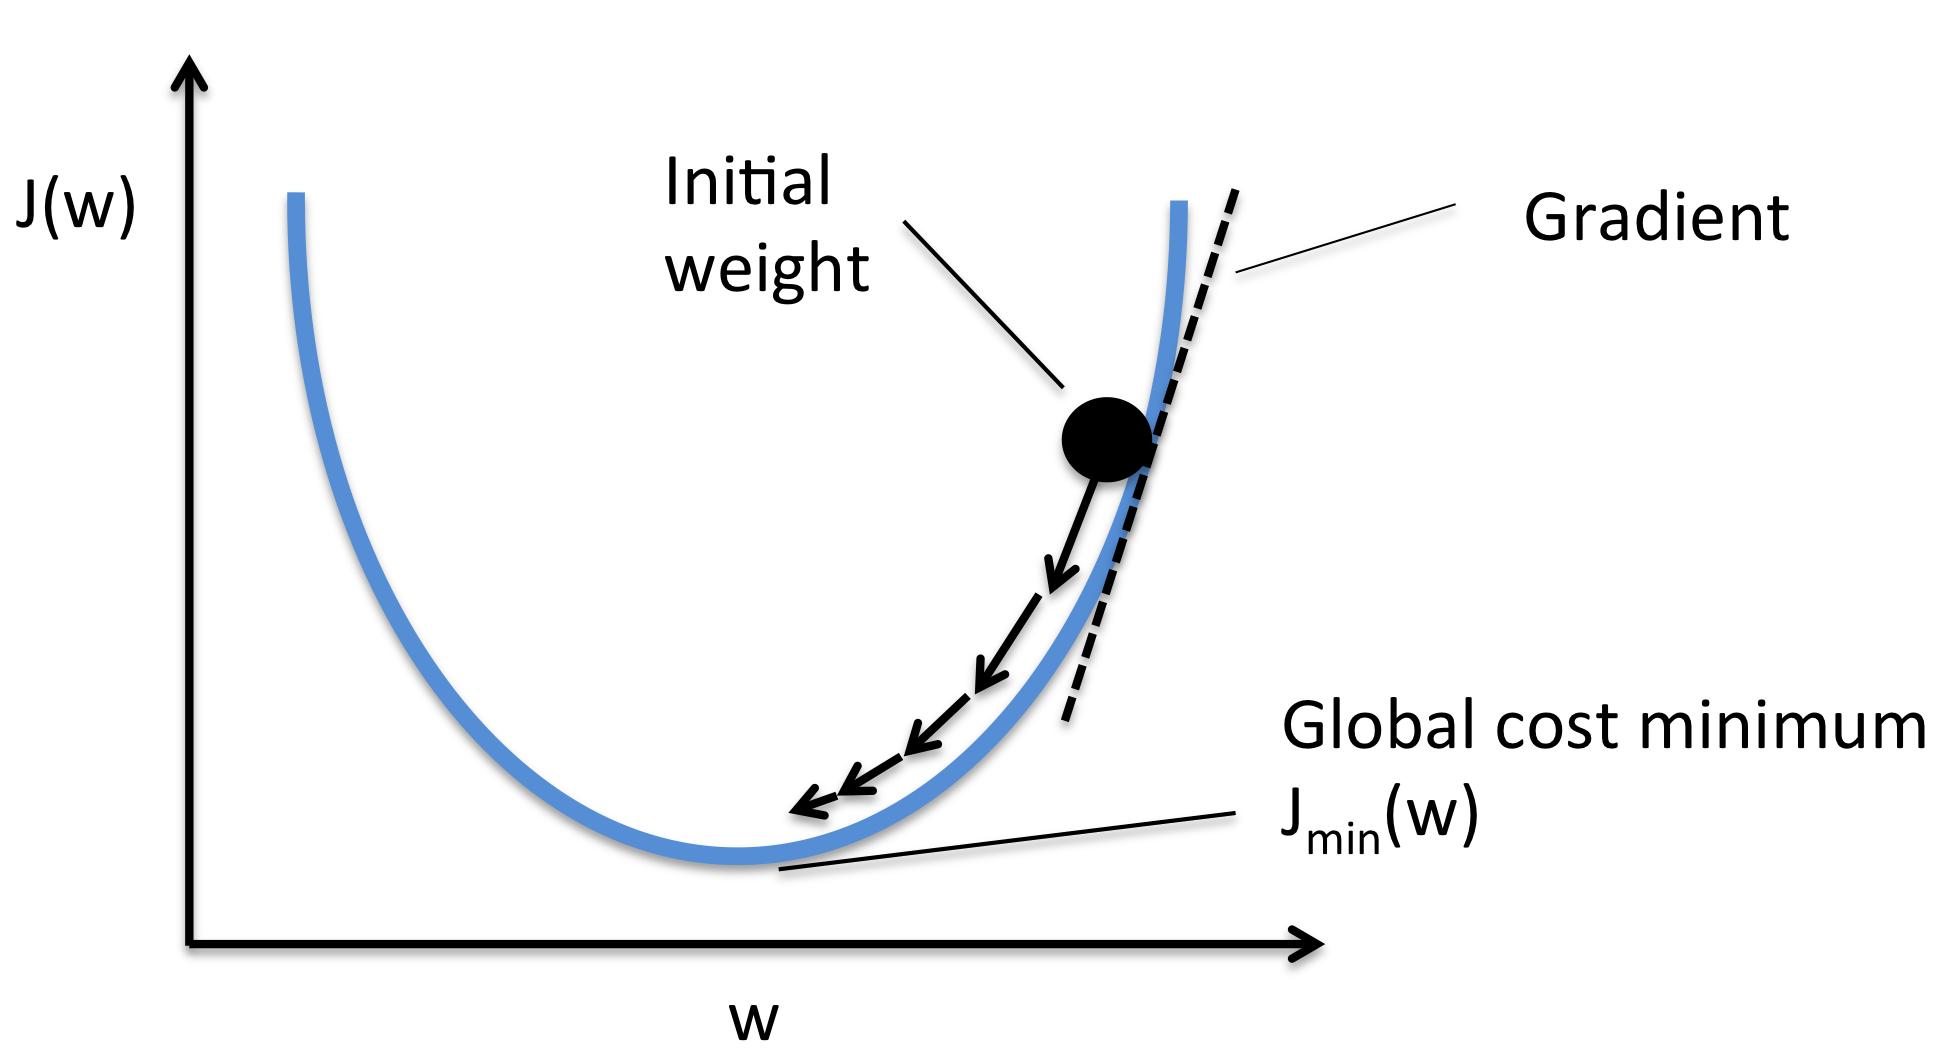
\includegraphics[width=.4\textwidth]{gradient-descend}
				\caption{Gradient descent}
				\label{fig:gradient-descend}
			\end{figure}

			\begin{equation}
				J(w) = \frac{1}{2} \sum_i (y^{(i)}-\phi(z^{(i)}))^2
			\end{equation}

			\paragraph{Update of weight vector}

			\begin{align}
					w_j &:= w_j + \Delta w_j \\
					\Delta w_j &= -\eta\nabla J(w) = \eta\sum_i (y^{(i)} -\phi(z^{(i)}))x^{(i)}_j
			\end{align}

			\paragraph{Features standarization}

			\begin{equation}
				x'_j = \frac{x_j - \mu_j}{\sigma_j}
			\end{equation}


			\subsubsection{Single Layer Neural Networks}
			\label{sec:single-layer-nn}


				\paragraph{Simple Perceptron}
				\label{sec:perceptron}
				[TODO ]

				\paragraph{ADALINE}
				\label{sec:adaline}
				[TODO ]

			\subsubsection{Multi Layer Perceptron}
			\label{sec:mlp}

				\paragraph{}
				[TODO ]

			\subsubsection{Radial Basis Functions}
			\label{sec:rbf}

				\paragraph{}
				[TODO ]

			\subsubsection{Convolutional Neural Networks}
			\label{sec:cnn}

				\paragraph{}
				[TODO ]

			\subsubsection{Recurrent Neural Networks}
			\label{sec:rnn}

				\paragraph{}
				[TODO ]

	\section{Unsupervised Learning}
	\label{sec:unsupervised-learning}

			\paragraph{}
			[TODO ]

%-----------------------------
%	Bibliographic references
%-----------------------------

	\nocite{subject:taa}
	\nocite{pactk:py-machine-learning}

  \bibliographystyle{alpha}
  \bibliography{bib}

\end{document}
